\documentclass[landscape,paper=160mm:90mm,fontsize=10pt,DIV=16]{scrartcl}

\newcommand{\docTitle}{Computer Recognition of Written Digits}
\newcommand{\docType}{Technical report}
\newcommand{\docDate}{2019-12-09}

\newcommand{\courseNumber}{BM40A0702}
\newcommand{\courseName}{Pattern Recognition and Machine Learning}

\newcommand{\authorA}{Noah Hellman}
\newcommand{\authorANum}{TODO123}
\newcommand{\authorB}{Viktor Dodonov}
\newcommand{\authorBNum}{TODO456}


% figures
\usepackage{graphicx}
\usepackage{subcaption}
\usepackage{color}
\usepackage{tikz}
\usepackage[top=8mm, bottom=0mm, left=7mm, right=7mm]{geometry}
\usetikzlibrary{matrix}

\pagestyle{empty}

\renewcommand{\familydefault}{\sfdefault}
\newenvironment{slide}[1]{\clearpage
    {\LARGE\bfseries#1\par}
}{}

\begin{document}

\begin{titlepage}
    \begin{center}
        \includegraphics[height=18mm]{doc/res/LUT-LOGO-CMYK-PDF.pdf}\\
        \vspace{3mm}
        {\small {\textsc{Lappeenranta University of Technology}}}\\
        \vspace{3mm}
        {\small {\textsc{\courseNumber{} - \courseName}}}\\
        \vfill
        {\bfseries \LARGE \docTitle}\\
        \vfill
        {\large \docDate}\\
        \vfill
        \def\tabcolsep{1.5cm}
        \begin{tabular}{lr}
            \textsc{\authorA} & \textsc{\authorB}
        \end{tabular}
        \vspace*{5mm}
    \end{center}
\end{titlepage}

\begin{slide}{Overview}
    \begin{itemize}
        \item Preproccessing
        \item Neural network (multilayer perceptron)
        \item Evaluation
    \end{itemize}
\end{slide}

\begin{slide}{Preprocessing}
    \vspace*{1cm}
    \begin{figure}[h]
        \centering
        \begin{subfigure}[c]{0.3\textwidth}
            \resizebox{\textwidth}{!}{\input{build/fig/preprocess_0.tex}}
            \caption{raw}
        \end{subfigure}%
        {\large $\rightarrow$}
        \begin{subfigure}[c]{0.3\textwidth}
            \resizebox{\textwidth}{!}{\input{build/fig/preprocess_1.tex}}
            \caption{projected}
        \end{subfigure}%
        {\large $\rightarrow$}
        \begin{subfigure}[c]{0.3\textwidth}
            \resizebox{\textwidth}{!}{\input{build/fig/preprocess_2.tex}}
            \caption{scaled and translated}
        \end{subfigure}
    \end{figure}
\end{slide}

\begin{slide}{Preprocessing}
    \vspace{1cm}
    \begin{figure}[h]
        \centering
        \begin{subfigure}[c]{0.3\textwidth}
            \centering
            \vspace*{-3.5mm}
            \resizebox{\textwidth}{!}{\input{build/fig/rasterize_0.tex}}
            \vspace*{-9mm}
            \caption{scaled}
        \end{subfigure}%
        {\large $\rightarrow$}
        \begin{subfigure}[c]{0.3\textwidth}
            \hspace*{4mm}
            \resizebox{0.92\textwidth}{!}{%
                \includegraphics{build/fig/rasterize_1.png}
            }
            \vfill
            \caption{rasterized}
        \end{subfigure}%
        {\large $\rightarrow$}
        \begin{subfigure}[c]{0.3\textwidth}
            \centering
            \hspace*{1mm}
            \resizebox{0.92\textwidth}{!}{%
                \includegraphics{build/fig/rasterize_2.png}
            }
            \vfill
            \caption{dilated}
        \end{subfigure}
    \end{figure}
\end{slide}

\begin{slide}{Neural network}
    \begin{minipage}{0.3\textwidth}
        \begin{itemize}
            \item 400 pixel intensities + bias as input neurons
            \item 1000 iterations of feedforward and backpropagation on 700
                training samples
            \item Multiple networks with different number of hidden neurons.
            \item Each classifier compared using a validation set (N=100).
        \end{itemize}
    \end{minipage}
    \begin{minipage}{0.7\textwidth}
        \vspace*{-5mm}
        \centering
        \resizebox*{\textwidth}{!}{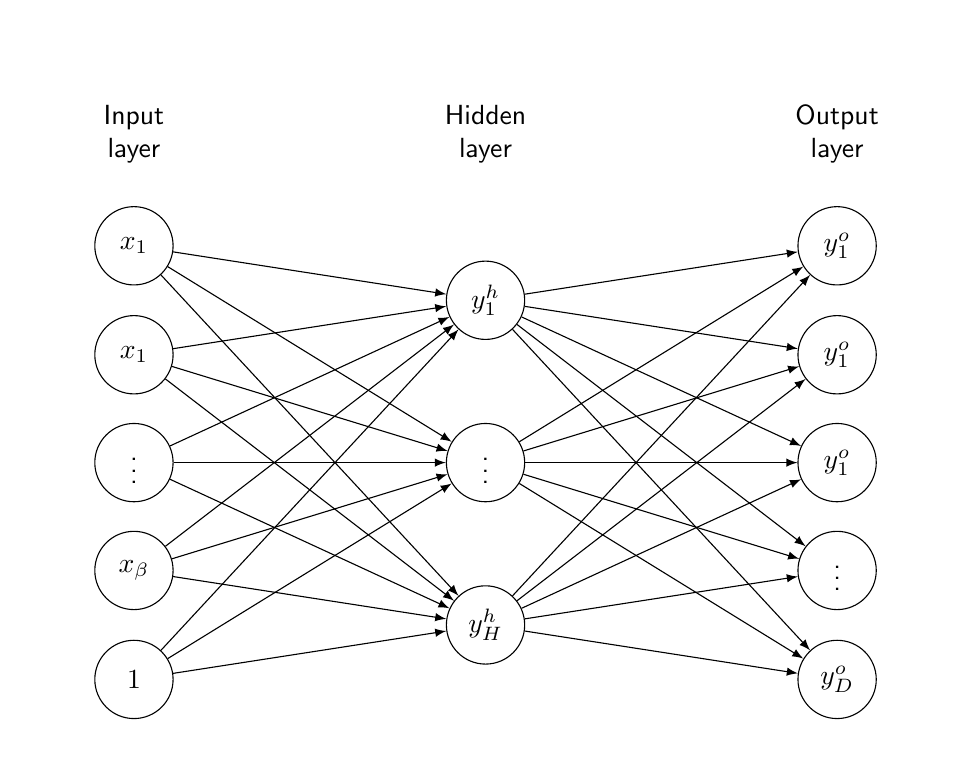
\begin{tikzpicture}[
    plain/.style={draw=none, fill=none},
    net/.style={
      matrix of nodes,
      nodes={draw, circle, inner sep=10pt},
      nodes in empty cells,
      column sep=2cm,
      row sep=-9pt
      },
    >=latex
    ]
    \matrix[net] (mat) {
        |[plain]| \parbox{1.3cm}{\centering Input layer} &
        |[plain]| \parbox{1.3cm}{\centering Hidden\\layer} &
        |[plain]| \parbox{1.3cm}{\centering Output\\layer} \\
                  & |[plain]| & \\
        |[plain]| &             \\
                  & |[plain]| & \\
        |[plain]| & |[plain]|   \\
                  &           & \\
        |[plain]| & |[plain]|   \\
                  & |[plain]| & \\
        |[plain]| &             \\
                  & |[plain]| & \\
    };

    % Neurons
    \foreach \ai in {2,4}
        \node at (mat-\ai-1) {$x_{1}$};
    \node at (mat-6-1) {$\vdots$};
    \node at (mat-8-1) {$x_{\beta}$};
    \node at (mat-10-1) {$1$};

    \node at (mat-3-2) {$y^h_1$};
    \node at (mat-6-2) {\vdots};
    \node at (mat-9-2) {$y^h_H$};

    \foreach \ai in {2,4,...,6}
        \node at (mat-\ai-3) {$y^o_1$};
    \node at (mat-8-3) {$\vdots$};
    \node at (mat-10-3) {$y^o_D$};

    % Weights
    \foreach \ai in {3,6,9}
        {\foreach \aii in {2,4,...,10}
            \draw[->] (mat-\ai-2) -- (mat-\aii-3);
        }

    \foreach \ai in {2,4,...,10}
        {\foreach \aii in {3,6,9}
            \draw[->] (mat-\ai-1) -- (mat-\aii-2);
        }
\end{tikzpicture}
}
    \end{minipage}
\end{slide}

\begin{slide}{Evaluation}
    \centering
    \begin{itemize}
        %\item 95\% of 100 validation samples correctly classified.
        \item 96.5\% of 200 test samples correctly classified.
    \end{itemize}
    \centering
    \resizebox*{0.9\textwidth}{!}{\input{build/fig/incorrect.tex}}
\end{slide}

\end{document}
